\documentclass[12pt,twoside,singlespace]{article}
\pagestyle{plain}

\usepackage{array, paralist, enumerate, amsmath, amsfonts, amssymb, amscd, color, mathrsfs,comment}
\usepackage{amsthm} % place after to make qedhere work
%\usepackage{times}
\usepackage{geometry}
\usepackage{framed}
\usepackage{hyperref}
\usepackage{graphicx}
\usepackage{epstopdf}
\usepackage[all,cmtip]{xy}
\usepackage{tikz}
\usepackage{tkz-graph}
\usetikzlibrary{arrows,%
                shapes,positioning}

\definecolor{DarkBlue}{rgb}{0,0,0.8} 
\definecolor{DarkGreen}{rgb}{0,0.5,0.0} 
\definecolor{DarkRed}{rgb}{0.9,0.0,0.0} 

\usepackage[T1]{fontenc}
\usepackage[latin1]{inputenc}
%\usepackage[inline]{showlabels}

\numberwithin{equation}{section}
\newtheorem{thm}[equation]{Theorem}
\newtheorem{lem}[equation]{Lemma}
\newtheorem{cor}[equation]{Corollary}
\newtheorem{prop}[equation]{Proposition}

\theoremstyle{definition}
\newtheorem{definition}[equation]{Definition}
\newtheorem{ex}[equation]{Example}	
\newtheorem{remark}[equation]{Remark}
\newtheorem{prob}{Problem}
\newtheorem{construction}[equation]{Construction}
\newtheorem{conjecture}[equation]{Conjecture}

\newcommand{\BB}{\mathbf{B}}
\newcommand{\ZZ}{\mathbf{Z}}
\newcommand{\NN}{\mathbf{N}}
\newcommand{\RR}{\mathbf{R}}
\newcommand{\QQ}{\mathbf{Q}}
\newcommand{\CC}{\mathbf{C}}
\newcommand{\FF}{\mathbf{F}}
\newcommand{\N}{N}
\newcommand{\po}[2]{\mathfrak{po}^{#1|#2}}
\newcommand{\on}{\operatorname}
\newcommand{\ra}{\rightarrow}
\newcommand{\ul}{\underline}
\newcommand{\ol}{\overline}
\newcommand{\nin}{\noindent}

\newcommand{\simple}{\text{simple}}
\newcommand{\Img}{\on{Im}}
\newcommand{\con}{\on{Con}}
\newcommand{\dash}{\on{Dash}}

\geometry{verbose,letterpaper,tmargin=1in}

\newcommand{\Q}{\overline{q}}
\newcommand{\w}{\on{weight}}

\newcommand{\val}{\on{Val}}
\newcommand{\smon}{\mathbf{SMon}}
\newcommand{\clif}{\on{clif}}
\newcommand{\cl}{\mathbf{Cl}}
%\newcommand{\mov}[2]{\on{mov}_{#2}(#1)}
\newcommand{\inc}{\on{inc}}
\newcommand{\cut}[4]{#1 = #2 \amalg_{#4} #3}
\newcommand{\cutr}[3]{#1 \amalg_{#3} #2}
%\newcommand{\piece}[3]{#1(#2|#3)}
\newcommand{\piece}[3]{#1_{#3}}
\newcommand{\wt}{\on{wt}}

\newcommand{\com}[1]{\textcolor{red}{$[\star \star \star$ #1 $\star \star \star]$}}

%%%%%%%%%%%%%%%%%%%%%%%%%%%%%% LyX specific LaTeX commands.
%% Bold symbol macro for standard LaTeX users
\providecommand{\boldsymbol}[1]{\mbox{\boldmath $#1$}}

%%%%%%%%%%%%%%%%%%%%%%%%%%%%%% User specified LaTeX commands.
\renewcommand{\vec}[1]{\mathbf{#1}}

%\renewcommand{\labelenumi}{(\alph{enumi})}
%\renewcommand{\labelenumii}{(\roman{enumii})}

%\usepackage{babel}

\title{Structural Theory of 2D Adinkras}
\author{Kevin Iga and Yan X Zhang}

\begin{document}

\pagestyle{plain}

\maketitle

\begin{abstract}
Adinkras are combinatorial objects developed to study supersymmetry representations. Most of the work so far on Adinkras apply to $1$-dimensional supersymmetry; in this paper, we give formal definitions and structural theorems for \emph{$2$-d Adinkras} to study $2$-dimensional supersymmetry. We show that the natural definitions we want (products, quotients, etc.) behave unexpectedly well, having a nice interplay with the classical theory of \emph{switching graphs}. Our main result is settling a conjecture of H\"ubsch, which helps us understand most of the structure of $2$-d Adinkras. The methods are mostly self-contained.
\end{abstract}


\section{Introduction}
Adinkras (in this paper, called $1$-d Adinkras) were introduced in \cite{d2l:first} to study representations of the super-Poincar\'e algebra in one dimension.  There have been a number of developments that have led to the classification of $1$-d Adinkras.\cite{d2l:graph-theoretic,d2l:omni,d2l:topology,zhang:adinkras,dil:cohomology,d2l:decodes}  Based on the success of this program, there have been a few recent approaches to using Adinkra-like ideas to study the super-Poincar\'e algebra in two dimensions.  This has led to the development of $2$-d Adinkras.\cite{gates:dimensional_extension,hubsch:weaving}

In this paper, we characterize $2$-d Adinkras.  At the core of this is the proof of a conjecture in \cite{hubsch:weaving}.  In the language we use in this paper, the theorem is as follows:

\begin{thm}
\label{thm:main}
Let $A$ be a connected $2$-d Adinkra.  Then there exist $1$-d Adinkras $A_1$ and $A_2$ so that
\[A\cong F(A_1\times A_2)/\sim\]
where $F$ is a vertex switch and  $\sim$ is described by an action of a subgroup of $\ZZ_2^n$.
\end{thm}

In \cite{hubsch:weaving}, the conjecture was phrased differently, and in Appendix~\ref{app:repn}, we explain the connection between these two formulations.

In this paper, we begin in Section~\ref{sec:prelim} by recalling the definition of $1$-d Adinkras and some of their features, including the code associated with an Adinkra and the concept of vertex switching.  In Section~\ref{sec:2d} we define a $2$-d Adinkra in the spirit of \cite{gates:dimensional_extension,hubsch:weaving}.  In Section~\ref{sec:products} we define how the product of two $1$-d Adinkras makes a $2$-d Adinkra, in the fashion described in the above theorem.  Section~\ref{sec:code2d} describes the codes for $2$-d Adinkras, called ESDE codes.  In Section~\ref{sec:quotient}, we prove the main theorem.  Then Section~\ref{sec:structure} demonstrates how the main theorem leads to understanding the basic structure of $2$-d Adinkras.

\section{Preliminaries}
\label{sec:prelim}

\subsection{$1$-d Adinkras}
\label{sec:1d}
\emph{Adinkras} in \cite{d2l:first,d2l:graph-theoretic,zhang:adinkras} will be referred to as \emph{$1$-d Adinkras} in this paper, since they relate to supersymmetry in $1$ dimension.  We will review a definition of $1$-d Adinkras now.

\begin{definition}[$1$-d Adinkras]
Let $n$ be a non-negative integer.  An \emph{$1$-d Adinkra} with $n$ colors is $(V,E,c,\mu,h)$ where
\begin{itemize}
\item $(V,E)$ is a finite undirected graph (called the \emph{underlying graph} of the Adinkra) with vertex set\footnote{In \cite{d2l:first,d2l:graph-theoretic}, there is also a bipartition of the vertices, where some vertices are represented by open circles and called bosons, and other vertices are represented by filled circles and called fermions.  This is not necessary to include in our definition, because the bipartition can be obtained directly by taking the grading $h$ modulo $2$, which is a bipartition by property 5 below.}
 $V$ and edge set $E$,
\item $c:E\to [n] := \{1,\ldots,n\}$ is a map called the \emph{coloring},
\item $\mu:E\to \ZZ_2=\{0,1\}$ is a map called the \emph{dashing},
\item $h:V\to\ZZ$ is a map called the \emph{grading}.
\end{itemize}

These are required to satisfy the following:
\begin{enumerate}
\item For every $v\in V$ and $c\in [n]$, there exist exactly one $w\in V$ so that $(v,w)\in E$ and $c(v,w)=c$. 
\item Every two-colored simple cycle must be of length 4.  (A \emph{simple} cycle is one which does not repeat vertices, with the exception of the start vertex equalling the end vertex.  A \emph{two-colored} cycle is one where the set of colors of the edges has cardinality $2$.)
\item The parity of $\mu$ on every two-colored simple cycle is odd; the \emph{parity} of $\mu$ on a cycle given by vertices $(v_0,\ldots,v_k)$ means the sum
\[\sum_{i=0}^{k-1}\mu(v_i,v_{i+1})\pmod{2}.\]
If a dashing $\mu$ satisfies this condition for all two-colored simple cycles, we call $\mu$ \emph{admissible}.
\item If $(v,w)\in E$, then $|h(v)-h(w)|=1$. Equivalently, $h$ provides a height function that makes $(V,E)$ into the Hasse diagram of a ranked poset.
\end{enumerate}

Figure~\ref{fig:1d-examples} give examples of $1$-d Adinkras.
\end{definition}


\begin{figure}
\begin{center}
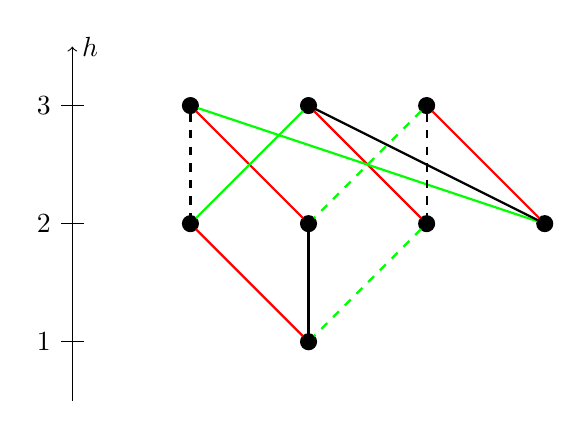
\begin{tikzpicture}[scale=0.15]
\SetVertexSimple[MinSize=5pt]
\SetUpEdge[labelstyle={draw}]
\Vertex[x=0,y=0]{A}
\Vertex[x=0,y=10]{B}
\Vertex[x=0,y=20]{C}
\Vertex[x=20,y=10]{D}
\Vertex[x=-10,y=10]{E}
\Vertex[x=10,y=10]{F}
\Vertex[x=-10,y=20]{G}
\Vertex[x=10,y=20]{H}
\Edge [color=red](G)(B)
\Edge[color=red](D)(H)
\Edge[color=red](C)(F)
\Edge[color=red](E)(A)
\Edge[color=green](D)(G)
\Edge[color=green, style=dashed](H)(B)
\Edge[color=green](C)(E)
\Edge[color=green, style=dashed](F)(A)
\Edge(D)(C)
\Edge[style=dashed](H)(F)
\Edge[style=dashed](G)(E)
\Edge(B)(A)
\draw [->] (-20,-5) -- (-20,25);
\draw (-19,0) -- (-21,0) node [align=right, left] {$1$};
\draw (-19,10) -- (-21,10) node [align=right, left] {$2$};
\draw (-19,20) -- (-21,20) node [align=right, left] {$3$};
\node [right] at (-20,25) {$h$};
\end{tikzpicture}
\caption{Examples of a $1$-d Adinkra with $3$ colors.  The grading function is represented by the vertical height as indicated on the axis on the left.
\label{fig:1d-examples}}
\end{center}
\end{figure}


\subsection{The action of $\ZZ_2^n$ and the code}
\label{sec:code}
The material in this section is mainly found in \cite{d2l:omni,zhang:adinkras}, with minor paraphrasing.  Let $A$ be a $1$-d Adinkra with $n$ colors, with vertex set $V$.  For all $i\in [n]$, define
\[q_i:V\to V\]
so that for all $v\in V$, $q_i(v)$ is the unique vertex joined to $v$ by an edge of color $i$.  In \cite{d2l:omni}, it was shown that the map $q_i$ is a graph isomorphism (in fact, an involution) from the underlying graph of $A$ to itself which preserves colors. The $q_i$ commute with each other. These facts can be used to combine the $q_1,\ldots, q_n$ maps into an action of $\ZZ_2^n$ on the graph $(V,E)$ underlying the Adinkra in the following way:
\begin{definition}
The action of $\ZZ_2^n$ on the graph $(V,E)$ underlying the Adinkra is given on vertices by
\[(x_1,\ldots,x_n)v=q_1^{x_1}\circ\cdots\circ q_n^{x_n}(v).\]
\end{definition}

Intuitively, the action of a sequence of bits, for instance, $11001$, on a vertex is obtained by following edges with colors that correspond to a $1$ (in this case, colors $1$, $2$, and $5$).  The fact that the $q_i$'s commute implies that the order of the colors does not matter.

The Adinkra $A$ is connected if and only if the $\ZZ_2^n$ action is transitive on the vertex set of $A$.  In this case the stabilizers of all vertices are equal (in general the stabilizers of two points in the same orbit are conjugate; here we know more since the group is abelian).  Define $C(A)$, the \emph{code of the Adinkra} $A$, to be this stabilizer.  As a subgroup of $\ZZ_2^n$, this is a binary block code of length $n$.  The code $C(A)$ is always a doubly-even code\cite{d2l:omni,d2l:decodes}, meaning that every codeword has a number of $1$s that is a multiple of $4$. It is a useful intuition to think of the underlying graph of an Adinkra as the quotient of the $n$-dimensional Hamming cube graph under such a code\cite{d2l:omni,zhang:adinkras}. This inspires us to think about using quotients later in Section~\ref{sec:quotient}.


\subsection{Vertex switching}
\label{sec:vertexswitch}

The following concept, somewhat ubiquitous in combinatorics under different guises, is first introduced in the context of Adinkras in \cite{d2l:first} and is more thoroughly set in its context in \cite{dil:cohomology,zhang:adinkras}.

\begin{definition}[Vertex switching]
Given an Adinkra $A$, and a vertex $v$ of $A$, we define \emph{vertex switching at $v$} to be the operation on $A$ that returns a new Adinkra $\bar{A}$ with the same vertices, edges, coloring, and grading but a new dashing $\bar{\mu}$ so that
\begin{equation}
\bar{\mu}(e)=\begin{cases}
1-\mu(e),&\mbox{if $e$ is incident to $v$}\\
\mu(e),&\mbox{otherwise.}
\end{cases}
\end{equation}
A vertex switching of $A$ is a composition of vertex switchings at various vertices of $A$.
\end{definition}

\begin{prop}
\label{prop:switching-still-adinkra}
If $A$ is an Adinkra, then so is $\bar{A}$.
\end{prop}
\begin{proof}
Since the vertices, edges, coloring, and grading(s) are the same, the only thing to check is the admissibility of $\bar{\mu}$.  This is straightforward and left to the reader.
\end{proof}

Douglas, Gates, and Wang \cite{douglas} examined dashings in Adinkras from a point of view inspired by Seidel's \emph{two-graphs} \cite{seidel:survey} \footnote{In Seidel's setting, \emph{vertex switching} switched the existence of edges, not the sign of edges; this can be seen as equivalent our definition applied to the complete graph. The type of vertex switching we do in this paper is sometimes called vertex switching on \emph{signed graphs} in literature for disambiguation.}. The second author \cite{zhang:adinkras} enumerated vertex switching classes and the number of dashings of $1$-d Adinkras.

\section{$2$-d Adinkras}
\label{sec:2d}
We would like to study $2$-d supersymmetry. The corresponding notion of what $2$-d Adinkras should be is described in \cite{gates:dimensional_extension,hubsch:weaving}.  We use a definition here that is equivalent to the one found there: the proof is found in Appendix \com{...[maybe?]}

A $2$-d Adinkra is similar to a $1$-d Adinkra except that some colors are called ``left-moving'' and the other colors called ``right-moving''.  Edges are called ``left-moving'' if they are colored by left-moving edges, and right-moving otherwise.  Furthermore, there are two gradings, one that is affected by the left-moving edges and the other for the right-moving edges. More formally,
\begin{definition}[$2$-d Adinkras]
Let $p$ and $q$ be non-negative integers. A \emph{2-d Adinkra} with $(p,q)$ colors is a 1-d Adinkra $(V,E,c,\mu,h)$ with $p+q$ colors, and two grading functions $h_L:V\to \ZZ$ and $h_R:V\to \ZZ$ so that
\begin{itemize}
\item $h(v)=h_L(v)+h_R(v)$.
\item Let $(v,w)\in E$.  If $c(v,w)\le p$ then $(v,w)$ is called a left-moving edge; if $c(v,w)>p$ then it is called a right-moving edge.
\item if $(v,w)$ is a left-moving edge, then $|h_L(v)-h_L(w)|=1$ and $h_R(v)=h_R(w)$.  If $(v,w)$ is a right-moving edge, then $|h_R(v)-h_R(w)|=1$ and $h_L(v)=h_L(w)$.
\end{itemize}

See Figure~\ref{fig:2d-example} for an example of a $2$-d Adinkra.
\end{definition}

\begin{figure}[htb]
\begin{center}
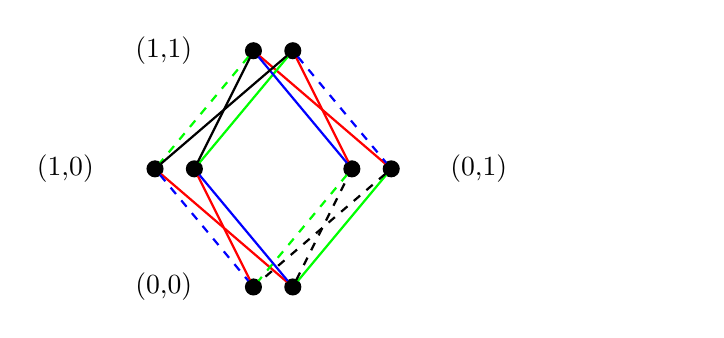
\begin{tikzpicture}[scale=0.05]
\SetVertexSimple[MinSize=5pt]
\node[text width=3cm] at (-10, 0) {(0,0)};
\node[text width=3cm] at (-35, 30) {(1,0)};
\node[text width=3cm] at (70, 30) {(0,1)};
\node[text width=3cm] at (-10, 60) {(1,1)};
\SetUpEdge[labelstyle={draw}]
\Vertex[x=0,y=0]{A}
\Vertex[x=-10,y=0]{H}
\Vertex[x=-35,y=30]{C}
\Vertex[x=-25,y=30]{B}
\Vertex[x=25,y=30]{D}
\Vertex[x=15,y=30]{E}
\Vertex[x=0,y=60]{G}
\Vertex[x=-10,y=60]{F}
\Edge[color=red](A)(C)
\Edge[color=red](B)(H)
\Edge[color=red](G)(E)
\Edge[color=red](F)(D)
\Edge[color=green](A)(D)
\Edge[color=green, style=dashed](E)(H)
\Edge[color=green](G)(B)
\Edge[color=green, style=dashed](F)(C)
\Edge[color=blue, style=dashed](C)(H)
\Edge[color=blue](B)(A)
\Edge[color=blue, style=dashed](G)(D)
\Edge[color=blue](F)(E)
\Edge[color=black, style=dashed](D)(H)
\Edge[color=black, style=dashed](A)(E)
\Edge[color=black](G)(C)
\Edge[color=black](B)(F)
\end{tikzpicture}
\caption{A $2$-d Adinkra with $(2,2)$ colors. The grading coordinates are given next to the nodes as $(h_L, h_R)$. \label{fig:2d-example}}
\end{center}
\end{figure}


\section{Products}
\label{sec:products}

We now begin to explore the structural theory of $2$-d Adinkras. It is desirable to have some way of combining Adinkras to make bigger ones (and conversely, breaking down bigger ones into smaller pieces). It is thus natural to consider defining products of Adinkras. With the right definition, it turns out that one way to get $2$-d Adinkras is to take a product of two $1$-d Adinkras, where the first Adinkra gives the left-moving colors and the second Adinkra gives the right-moving colors. We will eventually see in the next section that this operation (plus a quotient) is all we need to characterize a $2$-d Adinkra.

\begin{construction}
\label{const:product}
Let $p$ and $q$ be non-negative integers.  Let $A_1=(V_1, E_1, c_1, \mu_1,h_1)$ be a $1$-d Adinkra with $p$ colors and let $A_2=(V_2, E_2, c_2, \mu_2,h_2)$ be a $1$-d Adinkra $q$ colors.  We define the \emph{product} of these Adinkras $A_1\times A_2$ as the following 2-Adinkra with $(p,q)$ colors:
\[A_1\times A_2=(V,E,c,\mu,h_1,h_2)\]
where $V=V_1\times V_2$ and there are two kinds of edges in $E$:
\begin{itemize}
\item For every $(v_1,v_2)\in E_1$ and $w\in V_2$, we have an edge $((v_1,w),(v_2,w))$ of color $c_1(v_1,v_2)$ and dashing $\mu_1(v_1,v_2)$
\item For every $(w_1,w_2)\in E_2$ and $v\in V_1$, we have an edge $((v,w_1),(v,w_2))$ of color $p+c_2(w_1,w_2)$ and dashing
\begin{equation}
\label{eqn:dashprodshift}
\mu_2(w_1,w_2)+h_1(v)
\end{equation}
\end{itemize}
 See Figure~\ref{fig:product} for an example.
\end{construction}

\begin{figure}
\begin{center}
\begin{tabular}{c|c|c}
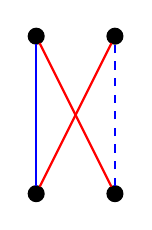
\begin{tikzpicture}[scale=0.1]
\SetVertexSimple[MinSize=5pt]
\SetUpEdge[labelstyle={draw}]
\Vertex[x=0,y=0]{A}
\Vertex[x=10,y=0]{B}
\Vertex[x=0,y=20]{E}
\Vertex[x=10,y=20]{F}
\Edge[color=blue](A)(E)
\Edge[color=blue, style=dashed](B)(F)
\Edge[color=red](A)(F)
\Edge[color=red](B)(E)
\end{tikzpicture}
&
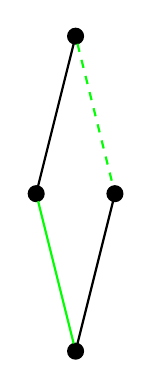
\begin{tikzpicture}[scale=0.1]
\SetVertexSimple[MinSize=5pt]
\SetUpEdge[labelstyle={draw}]
\Vertex[x=0,y=0]{A}
\Vertex[x=0,y=40]{B}
\Vertex[x=-5,y=20]{E}
\Vertex[x=5,y=20]{F}
\Edge[color=green](A)(E)
\Edge[color=green, style=dashed](B)(F)
\Edge[color=black](A)(F)
\Edge[color=black](B)(E)
\end{tikzpicture}
&
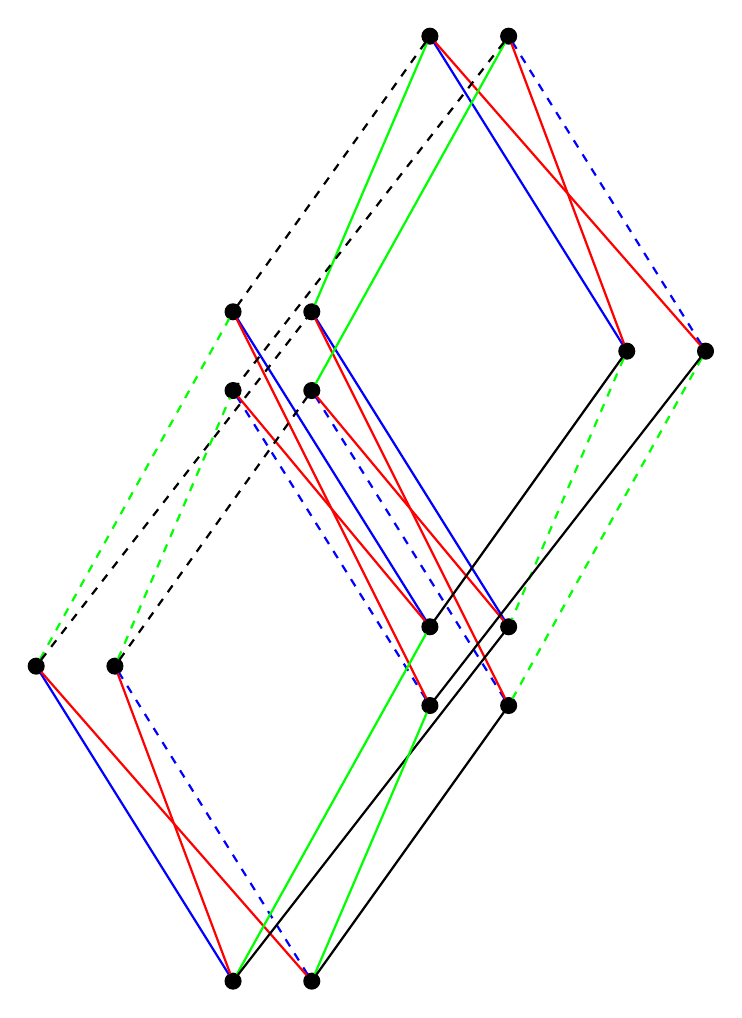
\begin{tikzpicture}[scale=0.1]
\SetVertexSimple[MinSize=5pt]
\SetUpEdge[labelstyle={draw}]
\Vertex[x=0,y=0]{BA}
\Vertex[x=-10,y=0]{AA}
\Vertex[x=-35,y=40]{EA}
\Vertex[x=-25,y=40]{FA}
\Vertex[x=25,y=45]{AF}
\Vertex[x=15,y=45]{AE}
\Vertex[x=0,y=85]{EF}
\Vertex[x=-10,y=85]{EE}
\Vertex[x=0,y=75]{FF}
\Vertex[x=-10,y=75]{FE}

\Vertex[x=40,y=80]{AB}
\Vertex[x=50,y=80]{BB}
\Vertex[x=15,y=120]{EB}
\Vertex[x=25,y=120]{FB}
\Vertex[x=25,y=35]{BF}
\Vertex[x=15,y=35]{BE}

\Edge[color=blue](AA)(EA)
\Edge[color=blue, style=dashed](BA)(FA)
\Edge[color=red](AA)(FA)
\Edge[color=red](BA)(EA)
\Edge[color=blue](AB)(EB)
\Edge[color=blue, style=dashed](BB)(FB)
\Edge[color=red](AB)(FB)
\Edge[color=red](BB)(EB)
\Edge[color=blue](AE)(EE)
\Edge[color=blue, style=dashed](BE)(FE)
\Edge[color=red](AE)(FE)
\Edge[color=red](BE)(EE)
\Edge[color=blue](AF)(EF)
\Edge[color=blue, style=dashed](BF)(FF)
\Edge[color=red](AF)(FF)
\Edge[color=red](BF)(EF)

\Edge[color=green](AA)(AE)
\Edge[color=green, style=dashed](AB)(AF)
\Edge[color=black](AA)(AF)
\Edge[color=black](AB)(AE)
\Edge[color=green](BA)(BE)
\Edge[color=green, style=dashed](BB)(BF)
\Edge[color=black](BA)(BF)
\Edge[color=black](BB)(BE)

\Edge[color=green, style=dashed](EA)(EE)
\Edge[color=green](EB)(EF)
\Edge[color=black, style=dashed](EA)(EF)
\Edge[color=black, style=dashed](EB)(EE)
\Edge[color=green, style=dashed](FA)(FE)
\Edge[color=green](FB)(FF)
\Edge[color=black, style=dashed](FA)(FF)
\Edge[color=black, style=dashed](FB)(FE)

\end{tikzpicture}
\end{tabular}
\caption{Constructing the $2$-d Adinkra from two smaller $1$-d Adinkras. Note that the dashings are all ``consistent'' with the smaller Adinkras, except for the right-moving edges on the upper-left ``boundary'' of the rectangle; these correspond to right-moving edges where the grading corresponding to the first Adinkra has height $1$.\label{fig:product}}
\end{center}
\end{figure}

This definition is intended to be a graph-theoretic version of the tensor product construction in $\ZZ_2$-graded representations (see Appendix~\ref{app:repn} for more details).  The edges that come from $E_1$ give rise to left-moving edges, and the edges that come from $E_2$ give rise to right-moving edges.  It follows easily that for every vertex $v$ in $A_1\times A_2$ and for every color in $[n]$ there is a unique edge in $A_1\times A_2$ incident to $v$.  The fact that two-colored simple cycles have length $4$ follows from following cases, depending on whether the colors are both left-moving, both right-moving, or one of each.  The parity condition for an Adinkra also follows from considering these cases.  The properties related to the bigrading are straightforward.  We then have:

\begin{prop}
\label{prop:product-admissable}
Given Adinkras $A_1$ and $A_2$, $A_1\times A_2$ is a $2$-d Adinkra.
\end{prop}


\begin{definition}[Extending codes]
Let $p$ and $q$ be non-negative integers and let $n=p+q$.  Define $Z_L:\ZZ_2^p\to\ZZ_2^n$ to be the function that appends $q$ zeros, so that for instance, if $p=4$ and $q=3$, then $Z_L(1011)=1011000$.  Likewise, define $Z_R:\ZZ_2^q\to\ZZ_2^n$ to be the function that prepends $p$ zeros.

Our most common use of this notation is as follows: if $C$ is a binary block code of length $p$, we write $Z_L(C)$ for the image under $Z_L$.  Likewise, if $C$ is a binary block code of length $q$, we write $Z_R(C)$ for the image under $Z_R$.
\end{definition}

\begin{prop}
\label{prop:prodcode}
Let $A_1$ and $A_2$ be as above.  Then
\[C(A_1\times A_2)=Z_L(C(A_1))\oplus Z_R(C(A_2)).\]
\end{prop}
\begin{proof}
Let $(v_1,v_2)\in A_1\times A_2$.  Let $\vec{x}\in \ZZ_2^N$.  We can write $\vec{x}=\vec{x}_L+\vec{x}_R$ where $\vec{x}_L$ is zero in the last $q$ bits and $\vec{x}_R$ is zero in the first $p$ bits.  Now
\[\vec{x}(v_1,v_2)=(\vec{x}_L+\vec{x}_R)(v_1,v_2)=(\vec{x}_Lv_1,\vec{x}_Rv_2).\]
This means that $\vec{x}(v_1,v_2)=(v_1,v_2)$ if and only if $\vec{x}_Lv_1=v_1$ and $\vec{x}_R v_2=v_2$. So $\vec{x}\in C(A_1\times A_2)$ if and only if $\vec{x}_L\in Z_L(C(A_1))$ and $\vec{x}_R\in Z_R(C(A_2))$.
\end{proof}

\section{Codes for $2$-d Adinkras}
\label{sec:code2d}
Let $A$ be a connected $2$-d Adinkra with $(p,q)$ colors.  Then there is a doubly even code $C(A)$ associated with $A$.  But as a $2$-d Adinkra, we make a distinction between the first $p$ colors and the last $q$ colors, which for a code translates to the first $p$ bits and the last $q$ bits.

For any vector $\vec{x}\in\ZZ_2^n$, the \emph{weight} of $\vec{x}$, denoted $\wt(\vec{x})$, is the number of $1$s in $\vec{x}$.  Likewise, $\wt_L(\vec{x})$ is the the number of $1$s in the first $p$ bits and $\wt_R(\vec{x})$ is the number of $1$s in the last $q$ bits of $\vec{x}$.

As was proved in \cite{hubsch:weaving}, if $A$ is a $2$-d Adinkra with $(p,q)$ colors and $C(A)$ is the code, then for every $\vec{x}\in C(A)$, we have that $\wt(\vec{x})$ is a multiple of $4$ and that both $\wt_L(\vec{x})$ and $\wt_R(\vec{x})$ are even.  Such a code is called \emph{even-split doubly even}, or \emph{ESDE}.  Thus, \cite{hubsch:weaving} proves the following theorem:
\begin{thm}
\label{thm:esde}
If $A$ is a connected $2$-d Adinkra with $(p,q)$ colors, then $C(A)$ is an ESDE.
\end{thm}

We now prove the converse of this theorem.  That is, given an ESDE code, there exist connected $2$-d Adinkra with that code.  This procedure is analogous to the Valise Adinkras in $1$-d,\cite{d2l:first,d2l:graph-theoretic} in that the possible values of each component $(h_L,h_R)$ of the bigrading is as small as possible, i.e., two values.

\begin{construction}
\label{cons:valise}
Let $K$ be an ESDE code.  We will describe a construction that provides a $2$-d Adinkra with code $C$, called the {\em Valise 2-d Adinkra}. First, since $C$ is doubly-even, there exists a connected $1$-d Adinkra $A$ with code $C(A) = C$. \cite{d2l:omni,d2l:topology} \com{(I think this kind of situation is exactly where it is best to have a concrete statement that the reader could refer to in section 2. -Y)} Fix a vertex $\overline{0}$ of $A$.  Now for every vertex $v$ there is a vector $\vec{x}\in\ZZ_2^n$ so that $\vec{x}\overline{0}=v$.  Then define $h_L(v)=\wt_L(\vec{x})\pmod{2}$ and $h_R(v)=\wt_R(\vec{x})\pmod{2}$.  Note that these functions are well-defined since $C$ is ESDE.  Then $(h_L, h_R)$ is a bigrading for $A$, making it a $2$-d Adinkra.  An example of the kind of $2$-d Adinkra that arises from this construction is Figure~\ref{fig:2d-example}.
\end{construction}

We therefore have:
\begin{thm}
\label{thm:esde}
For a code $C \subset \ZZ_2^n$, there exists a $2$-d Adinkra $A$ with $C(A) = C$ if and only if $C$ is a ESDE code.
\end{thm}




The structure of the ESDE relates to interesting features of the colored graph of $A$.  Let $A_L$ be the $1$-d Adinkra with $p$ colors that consists of only the left-moving edges of $A$.  Let $A_R$ be the $1$-d Adinkra with $q$ colors that consists of only the right-moving edges of $A$ (where we shift the colors so that they range from $1$ to $q$ instead of $p+1$ to $p+q$).  Pick a vertex $\overline{0}$ in $A$.  Let $A_L^0$ be the connected component of $A_L$ containing $\overline{0}$ and let $A_R^0$ be the connected component of $A_R$ containing $\overline{0}$.

We now see that the codes for $A_L^0$ and $A_R^0$ (with an appropriate number of $0$s added to the left or right as necessary) provide important linear subspaces of $C(A)$.

\begin{prop}
\[Z_L(C(A_L^0))=C(A)\cap Z_L(\ZZ_2^p)\]
\[Z_R(C(A_R^0))=C(A)\cap Z_R(\ZZ_2^q)\]
\end{prop}
In other words, the codewords that are zero in the last $q$ bits are precisely the codewords from $C(A_L^0)$ with $q$ zeros appended to the right; and the codewords that are zero in the first $p$ bits are precisely the codewords from $C(A_R^0)$ with $p$ zeros prepended to the left.
\begin{proof}
If $\vec{x}\in Z_L(C(A_L^0))$, so that $\vec{x}=Z_L(\vec{y})$ for some $\vec{y}\in C(A_L^0)$.  Then trivially $\vec{x}\in Z_L(\ZZ_2^p)$.  Furthermore, $\vec{y}\overline{0}=\overline{0}$ in $A_L^0$.  In $A$, $Z_L(\vec{y})=\vec{x}$ does exactly the same thing, so $\vec{x}\overline{0}=\overline{0}$ in $A$.  Therefore $\vec{x}\in C(A)$.

Conversely if $\vec{x}\in C(A)\cap Z_L(\ZZ_2^p)$, then by the definition of the group action there is a path in $A$ from $\overline{0}$ to $\overline{0}$ following the colors corresponding to the $1$s in $\vec{x}$.  Since $\vec{x}\in Z_L(\ZZ_2^p)$, we have that this path only consists of left-moving colors, and so lies in $A_L^0$.

The proof for $Z_R(C(A_R^0))$ is similar.
\end{proof}

\begin{cor}
\label{cor:cplus}
\[Z_L(C(A_L^0))\oplus Z_R(C(A_R^0))\subset C(A)\]
\end{cor}
Comparing with Proposition~\ref{prop:prodcode}, this corollary says that the code for $A_L^0\times A_R^0$ is a linear subspace of the code for $A$.

Simply for brevity (and thus, readability) in later descriptions, we define using the product construction above $A'=A_L^0\times A_R^0$, and the code $C'=Z_L(C(A_L^0))\oplus Z_R(C(A_R^0))$.  Also, we write $C$ for $C(A)$.  Then $C(A')=C'$ and $C'\subset C$.

\begin{lem}
\label{lem:existk}
There exists a binary linear block code $K$ so that
\[C=C' \oplus K.
\]
\end{lem}
\begin{proof}
From Corollary~\ref{cor:cplus} and basic linear algebra, there exists a vector subspace $K$ of $\ZZ_2^n$ that is a vector space complement of
$C'$ in $C$.
\end{proof}
Note that $K$ is not necessarily uniquely defined.  It is, however, uniquely defined up to adding vectors in $C'$.  So a more invariant approach would be to use $C/C'$ instead of $K$, but $K$ has the advantage of being a code, therefore more concrete for computational purposes.



The interpretation of $K$ can be obtained by examining the set $V^0=A_L^0\cap A_R^0$.  Since $A_L^0$ has only left-moving edges and $A_R^0$ has only right-moving edges, $V^0$ has no edges at all: only vertices.  Furthermore, for every $v\in V^0$, we have $h_L(v)=h_L(\overline{0})$ and $h_R(v)=h_R(\overline{0})$ so all of the vertices in $V^0$ have the same bigrading.

We now show that there is a bijection between $K$ and $V^0$.

As before, for every $\vec{x}\in\ZZ_2^n$, we write $\vec{x}=\vec{x}_L+\vec{x}_R$, where $\vec{x}_L$ is zero in the last $q$ bits and $\vec{x}_R$ is zero in the first $p$ bits.  Using this notation, we have the following theorem.

\begin{thm}
\label{thm:kv0}
The map
\[\Psi:K\to V^0\]
given by
\[\Psi(\vec{x})=\vec{x}_L\overline{0}\]
is a bijection.
\end{thm}
\begin{proof}
If $\vec{x}\in K\subset C(A)$, then $(\vec{x}_L+\vec{x}_R)\overline{0}=\overline{0}$, so $\vec{x}_L\overline{0}=\vec{x}_R\overline{0}$.  So $\Psi(\vec{x})\in A_L^0\cap A_R^0=V^0$.

To prove $\Psi$ is one-to-one, suppose $\Psi(\vec{x})=\Psi(\vec{y})$.  Then $\vec{x}_L\overline{0}=\vec{y}_L\overline{0}$.  Therefore $\vec{x}_L+\vec{y}_L\in C(A_L^0)$.  Likewise $\vec{x}_R+\vec{y}_R\in C(A_R^0)$.  So $\vec{x}+\vec{y}\in C'$.  Since $C'\cap K=\{\vec{0}\}$, we have that $\Psi$ is one-to-one.

To prove $\Psi$ is onto, let $v\in V^0$.  Since $v\in A_L^0$, there exists $\vec{x}_L$ with last $q$ bits zero, so that $\vec{x}_L\overline{0}=v$ in $A_L^0$.  Likewise there exists $\vec{x}_R$ with first $p$ bits zero, so that $\vec{x}_R\overline{0}=v$ in $A_R^0$.  Then $\vec{x}=\vec{x}_L+\vec{x}_R\in C(A)$.  Since $C(A)=C'\oplus K$, we can write $\vec{x}=\vec{c}+\vec{k}$ where $\vec{c}\in C'$ and $\vec{k}\in K$.  By the fact that $C'=Z_L(C(A_L^0))\oplus Z_R(C(A_R^0))$, we have that $\vec{c}_L\in Z_L(C(A_L^0))$ and so $\vec{c}_L\overline{0}=\overline{0}$.  Then
$\Psi(\vec{k})=\vec{k}_L\overline{0}
=(\vec{x}_L-\vec{c}_L)\overline{0}
=\vec{x}_L(\vec{c}_L(\overline{0}))
=\vec{x}_L(\overline{0})
=v.$
\end{proof}


Consider the following examples.
\begin{ex}
Let $p=4$ and $q=2$ and the generating matrix for $C$ be
\[\left[\begin{array}{cccc|cc}
1&1&1&1&0&0\\
0&0&1&1&1&1
\end{array}\right].\]
Then $Z_L(C(A_L^0))$ has generating vector $\vec{m} = \left[\begin{array}{cccc|cc}
1&1&1&1&0&0\\
\end{array}\right]$ and $Z_R(C(A_R^0))=\{\vec{0}\}$, the trivial code.  We therefore see that $A_L^0$ is a $1$-d Adinkra with four colors with code with generating vector
$\left[\begin{array}{cccc}
1&1&1&1\\
\end{array}\right]$ and $A_R^0$ is a $1$-d Adinkra with two colors with trivial code.  The code $K$ can be chosen to be generated by $\vec{k} = \left[\begin{array}{cccc|cc}
0&0&1&1&1&1
\end{array}\right]$. Another choice for $K$ would have been the code generated by 
\[\vec{k} + \vec{m} = \left[\begin{array}{cccc|cc}
1&1&0&0&1&1
\end{array}\right].\]

See Figure~\ref{fig:example-quotient} for this example. To use Theorem~\ref{thm:kv0}, we start at $\overline{0}$ and follow an edge of color $3$, then an edge of color $4$, which uses the left-moving edges in $001111$.  This brings us to a new vertex, which is in $V^0$.  This vertex, and $\overline{0}$ itself, are the two elements of $V^0$, corresponding to the two elements of $K$. 
\end{ex}

\begin{figure}
\begin{center}
\begin{tabular}{c}
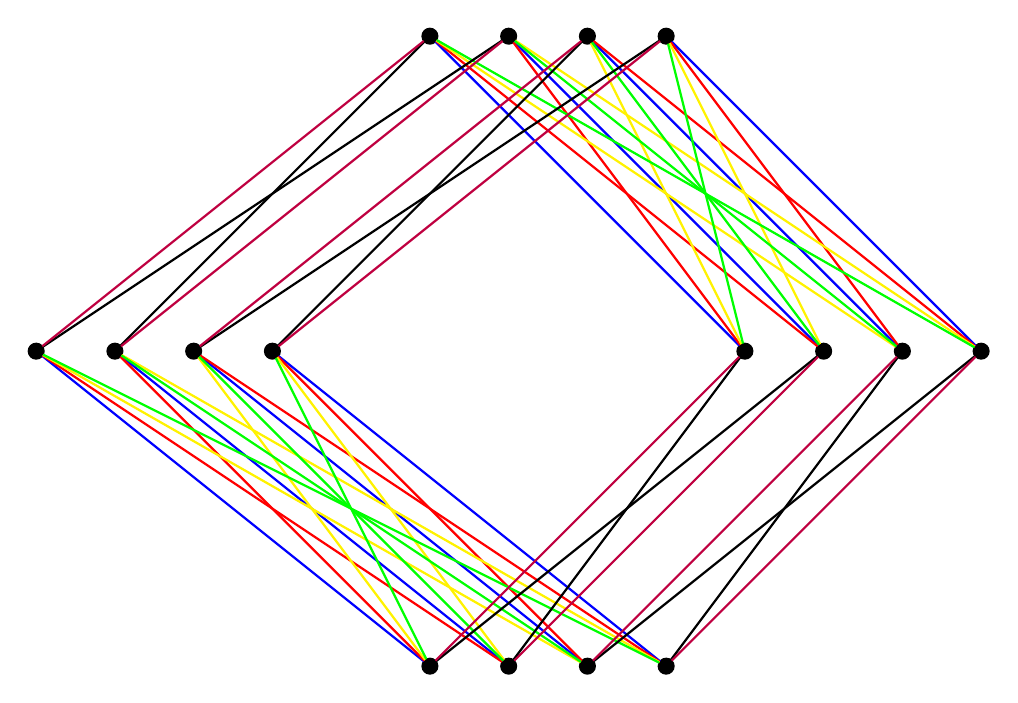
\begin{tikzpicture}[scale=0.1]
\SetVertexSimple[MinSize=5pt]
\SetUpEdge[labelstyle={draw}]
\Vertex[x=0,y=0]{000000}
\Vertex[x=-50,y=40]{000100}
\Vertex[x=-40,y=40]{001000}
\Vertex[x=10,y=0]{001100}
\Vertex[x=-30,y=40]{010000}
\Vertex[x=20,y=0]{010100}
\Vertex[x=30,y=0]{011000}
\Vertex[x=-20,y=40]{011100}
\Vertex[x=40,y=40]{000001}
\Vertex[x=0,y=80]{000101}
\Vertex[x=10,y=80]{001001}
\Vertex[x=50,y=40]{001101}
\Vertex[x=20,y=80]{010001}
\Vertex[x=60,y=40]{010101}
\Vertex[x=70,y=40]{011001}
\Vertex[x=30,y=80]{011101}

\Edge[color=blue](000000)(000100)
\Edge[color=blue](001000)(001100)
\Edge[color=blue](010000)(010100)
\Edge[color=blue](011000)(011100)
\Edge[color=blue](000001)(000101)
\Edge[color=blue](001001)(001101)
\Edge[color=blue](010001)(010101)
\Edge[color=blue](011001)(011101)

\Edge[color=red](000000)(001000)
\Edge[color=red](000100)(001100)
\Edge[color=red](010000)(011000)
\Edge[color=red](010100)(011100)
\Edge[color=red](000001)(001001)
\Edge[color=red](000101)(001101)
\Edge[color=red](010001)(011001)
\Edge[color=red](010101)(011101)

\Edge[color=yellow](000000)(010000)
\Edge[color=yellow](011100)(001100)
\Edge[color=yellow](000100)(010100)
\Edge[color=yellow](011000)(001000)
\Edge[color=yellow](000001)(010001)
\Edge[color=yellow](001001)(011001)
\Edge[color=yellow](000101)(010101)
\Edge[color=yellow](001101)(011101)

\Edge[color=green](000000)(011100)
\Edge[color=green](001000)(010100)
\Edge[color=green](010000)(001100)
\Edge[color=green](011000)(000100)
\Edge[color=green](000001)(011101)
\Edge[color=green](001001)(010101)
\Edge[color=green](010001)(001101)
\Edge[color=green](011001)(000101)

\Edge[color=black](000000)(001101)
\Edge[color=black](000100)(001001)
\Edge[color=black](010000)(011101)
\Edge[color=black](010100)(011001)
\Edge[color=black](000001)(001100)
\Edge[color=black](000101)(001000)
\Edge[color=black](010001)(011100)
\Edge[color=black](010101)(011000)

\Edge[color=purple](000000)(000001)
\Edge[color=purple](000100)(000101)
\Edge[color=purple](010000)(010001)
\Edge[color=purple](010100)(010101)
\Edge[color=purple](001000)(001001)
\Edge[color=purple](001100)(001101)
\Edge[color=purple](011000)(011001)
\Edge[color=purple](011100)(011101)
\end{tikzpicture} \\
\hline
\begin{tabular}{l|r}
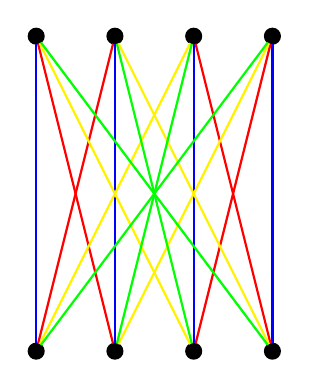
\begin{tikzpicture}[scale=0.1]
\SetVertexSimple[MinSize=5pt]
\SetUpEdge[labelstyle={draw}]
\Vertex[x=0,y=0]{000000}
\Vertex[x=0,y=40]{000100}
\Vertex[x=10,y=40]{001000}
\Vertex[x=10,y=0]{001100}
\Vertex[x=20,y=40]{010000}
\Vertex[x=20,y=0]{010100}
\Vertex[x=30,y=0]{011000}
\Vertex[x=30,y=40]{011100}

\Edge[color=blue](000000)(000100)
\Edge[color=blue](001000)(001100)
\Edge[color=blue](010000)(010100)
\Edge[color=blue](011000)(011100)
\Edge[color=red](000000)(001000)
\Edge[color=red](000100)(001100)
\Edge[color=red](010000)(011000)
\Edge[color=red](010100)(011100)
\Edge[color=yellow](000000)(010000)
\Edge[color=yellow](011100)(001100)
\Edge[color=yellow](000100)(010100)
\Edge[color=yellow](011000)(001000)
\Edge[color=green](000000)(011100)
\Edge[color=green](001000)(010100)
\Edge[color=green](010000)(001100)
\Edge[color=green](011000)(000100)
\end{tikzpicture} & 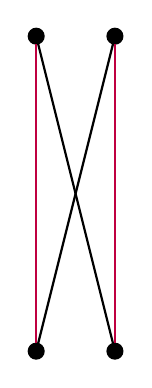
\begin{tikzpicture}[scale=0.1]
\SetVertexSimple[MinSize=5pt]
\SetUpEdge[labelstyle={draw}]
\Vertex[x=0,y=0]{000000}
\Vertex[x=10,y=0]{001100}
\Vertex[x=0,y=40]{000001}
\Vertex[x=10,y=40]{001101}
\Edge[color=black](000000)(001101)
\Edge[color=black](000001)(001100)
\Edge[color=purple](000000)(000001)
\Edge[color=purple](001100)(001101)
\end{tikzpicture}
\end{tabular} 
\end{tabular}
\end{center}
\caption{Top: a $2$-d Adinkra with dashes omitted. Bottom: picking any vertex and looking at connected components give us a pair of $1$-d Adinkras $A_L^0$ and $A_R^0$, the product of which contains as a quotient the original Adinkra; in this case we quotient via a $1$-dimensional code of size $2^1 = 2$, obtaining $8 \times 4 / 2 = 16$ vertices, as desired.  \label{fig:example-quotient}}
\end{figure}


\begin{ex}
Let $p=q=4$ and consider the following generating matrix for $C$:
\[\left[\begin{array}{cccc|cccc}
1&1&0&0&1&1&0&0\\
1&1&1&1&1&1&1&1\\
0&0&1&1&1&1&0&0\\
1&0&1&0&1&0&1&0
\end{array}\right]\]
If we let $\vec{x}_1, \ldots, \vec{x}_4$ be the rows of this matrix, we see that $\vec{x}_1+\vec{x}_3$ has zeros on the right side of the vertical line.  Other than the zero word, no other combination has all zeros on the right side, so $Z_L(C(A_L^0))$ has generating matrix
\[\left[\begin{array}{cccc|cccc}
1&1&1&1&0&0&0&0
\end{array}\right]\]
and $C(A_L^0)$ has generating matrix
\[\left[\begin{array}{cccc}
1&1&1&1
\end{array}\right].\]
Likewise we can find $\vec{x}_1+\vec{x}_2+\vec{x}_3$ which is the unique nonzero codeword with all zeros on the left side, and so $Z_R(C(A_R^0))$ has generating matrix
\[\left[\begin{array}{cccc|cccc}
0&0&0&0&1&1&1&1
\end{array}\right]\]
and $C(A_R^0)$ has generating matrix
\[\left[\begin{array}{cccc}
1&1&1&1
\end{array}\right].\]
Then $A_L^0$ and $A_R^0$ are both $1$-d Adinkras with $4$ colors with code generated by $1111$, and $K$ can be taken to be (for instance)
\[\left[\begin{array}{cccc|cccc}
0&0&1&1&1&1&0&0\\
1&0&1&0&1&0&1&0
\end{array}\right].\]
Standard arguments in linear algebra allow us to choose the generating basis for $C$ to consist of a generating basis for $Z_L(C(A_L^0))$, then a generating basis for $Z_R(C(A_R^0))$, then a generating basis for $K$.  In this case, we would write
\[\left[\begin{array}{cccc|cccc}
1&1&1&1&0&0&0&0\\\hline
0&0&0&0&1&1&1&1\\\hline
0&0&1&1&1&1&0&0\\
1&0&1&0&1&0&1&0
\end{array}\right]\]
where the horizontal lines separate the three subspaces.  Each line has weight a multiple of $4$, where the first two lines have the $1$s all on one side or the other, while the last two lines (the ones responsible for $K$) have the $1$s split on both sides in a way that both sides have even weight.

Then $V^0$ has four elements: $\overline{0}$, $(00110000)\overline{0}$, $(10100000)\overline{0}$, and $(10010000)\overline{0}$.

\com{Should we draw a $2$-d Adinkra for this?}
\end{ex}


\subsection{Classifying ESDE codes}
While not necessary for proving the main theorem of this paper, \cite{hubsch:weaving} also asked how to classify ESDE codes.  To do this, it is useful to extend the notion of the splitting of $n$ into $p+q$.  In particular, instead of insisting that the left-moving colors be written as the first $p$ bits, we partition $[n]$ into $[n]=L\cup R$ such that $|L|=p$ and $|R|=q$.  We fix $n$ and a doubly even code $C$, then characterize which partitions into $L$ and $R$ make $C$ an ESDE.

\begin{thm}
\label{thm:esde}
Given a doubly even code $C$ of length $n$, there is a bijection between codewords in $C^\perp$ and (ordered) paritions $L \cup R$ that make $C$ into an ESDE. There are $2^{n-k}$ such partitions. 
\end{thm}
\begin{proof}
Consider a partition $L \cup R$ that makes $C$ into an ESDE, and consider the codeword $w$ that is defined to have $1$ at all the positions in $L$ and $0$ at all the positions in $R$.  By definition of ESDE codes, all codewords in $C$ have an even number of $1$'s in the support of $w$, which is equivalent to saying that $w$ is orthogonal to all the codewords in $C$. Thus, $w \in C^\perp$.  Conversely, for any $w \in C^\perp$, $w$ is orthogonal to all codewords in $C$ and thus give an ESDE. Thus, there is a bijection between the two sets.  Note these are ordered partitions; the codeword which has $1$ at all the positions in $R$ and $0$ otherwise would give the same paritition, but in reversed order.
\end{proof}

\section{Proof of main theorem}
\label{sec:quotient}
In this section we prove the main theorem of the paper, Theorem~\ref{thm:main}.  This refers to a connected $2$-d Adinkra $A$ with $(p,q)$ colors.  As in Section~\ref{sec:code2d} we pick a vertex $\overline{0}$ in $A$ and define $A_L^0$, $A_R^0$.  We use Construction~\ref{const:product} to define $A'=A_L^0\times A_R^0$ and let $C=C(A)$ and $C'=C(A')=Z_L(C(A_L^0))\oplus Z_R(C(A_R^0))$.  Let $K$ be a code given by Lemma~\ref{lem:existk}.

The main result is
\begin{thm}
\label{thm:quotient}
Let $A$ be a connected $2$-d Adinkra.  Then there is a vertex switch $F$ and an action of $K$ on $F(A')$ that preserves colors, dashing, and bigrading, and so that
\[F(A')/K\cong A\]
as an isomorphism of $2$-d Adinkras (that is, as an isomorphism of graphs that preserves colors, dashing, and bigrading).
\end{thm}

We prove Theorem~\ref{thm:quotient} in two steps, by first constructing a (color and bigrading preserving) graph isomorphism $\tilde{\Phi}:A'/K\to A$ and then finding a suitable vertex switch $F$.

\begin{thm}
\label{thm:isocolors}
The code $K$ acts on $A'$ via color preserving isomorphisms to produce a quotient $A'/K$.  There is a color preserving graph epimorphism $\Phi:A' \to A$ that sends $(\overline{0},\overline{0})$ to $\overline{0}$.  This descends to $A'/K$ to produce a color preserving graph isomorphism $\tilde{\Phi}:A'/K\to A$.
\end{thm}
\begin{proof}
Let $I^n$ be the colored Hamming cube: that is, a graph with vertex set $\{0,1\}^n$ and two vertices are connected with an edge of color $i$ if they differ only in bit $i$.  Recall that every connected Adinkra is, as a colored graph, the quotient of $I^n$ by the code for the Adinkra.\cite{d2l:omni}  So we have $I^n/C \cong A$ and $I^n/C'\cong A'$. These are isomorphisms as colored graphs.  They can be chosen so that $\vec{0}=(0,\ldots,0)$ is sent to $\overline{0}$ in $A$ and $(\overline{0},\overline{0})$ in $A'$, respectively.

Now $K$ is a doubly even code, and $K\cap C'=0$, so $K$ acts on $I^n/C'$ and on $A'$ in a way that nontrivial elements of $K$ move vertices a distance greater than $2$.  By \cite{zhang:adinkras}, this means we can quotient the colored graph $I^n/C'$, and thus $A'$, by $K$.  We then have the following commutative diagram of colored graphs:

\[
\begin{CD}
I^n/C' @>i_1>\cong> A'\\
@VV\pi_1 V @VV\pi_2 V\\
(I^n/C')/K @>i_2>\cong> A'/K\\
\end{CD}  
\]

A standard argument gives
\[(I^n/C')/K \cong I^n/(C'\oplus K)=I^n/C,\]
and adding this to the above commutative diagram, we then have:
\[
\xymatrixcolsep{5pc}
\xymatrix{
I^n/C' \ar[d]^{\pi_1} \ar[r]^{i_1}_{\cong} &A'\ar[d]^{\pi_2}\ar@/^2pc/[dd]^{\Phi} \\
(I^n/C')/K \ar[d]^{i_4}_{\cong} \ar[r]^{i_2}_\cong &A'/K\ar[d]_{\cong}^{\tilde{\Phi}}\\
I^n/(C'\oplus K) \ar[r]^{i_3}_\cong &A.}
\]
where $\tilde{\Phi}=i_3\circ i_4\circ i_2^{-1}$ and $\Phi=\tilde{\Phi}\circ \pi_2$.  Then $\tilde{\Phi}$ is an isomorphism of colored graphs, and $\Phi$ is an epimorphism of colored graphs.  Standard diagram chasing shows that $\Phi(\overline{0},\overline{0})=\overline{0}$.
\end{proof}

It will be useful to have the following result:
\begin{lem}
\label{lem:gphi}
If $\vec{x}\in \ZZ_2^n$, then $\Phi(\vec{x}(v_1,v_2))=\vec{x}\Phi(v_1,v_2).$
\end{lem}
\begin{proof}
For $\vec{x}=\vec{e}_i$, the vector that is $1$ in component $i$ and $0$ otherwise, this lemma is the statement that $\Phi$ is color-preserving.  By composing many maps of this type, we get the statement for all vectors $\vec{x}\in \ZZ_2^n$.
\end{proof}

\begin{lem}
\label{lem:phisides}
For all $v\in A_L^0$, $\Phi(v,\overline{0})=v$, and for all $w\in A_R^0$, $\Phi(\overline{0},w)=w$.  In particular, $\Phi$ restricted to $A_L^0\times\{\overline{0}\}$ is an isomorphism onto its image, and likewise for $\Phi$ restricted to $\{\overline{0}\}\times A_R^0$.
\end{lem}
\begin{proof}
Let $\vec{x}\in \ZZ_2^p$ be such that $\vec{x}\overline{0}=v$.  By Lemma~\ref{lem:gphi}, $\Phi(v,0) = \Phi(Z_L(\vec{x})(\overline{0},\overline{0})) = Z_L(\vec{x})\Phi(\overline{0},\overline{0})=Z_L(\vec{x})\overline{0}=v$.  The proof for $w$ is similar.
\end{proof}

\begin{lem}
\label{lem:phiformula}
Let $(v,w)\in A'$, with $w=\vec{x}\overline{0}$.  Then
\[\Phi(v,w)=Z_R(\vec{x})v.\]
\end{lem}
\begin{proof}
We have
\[\Phi(v,\overline{0})=v\]
from Lemma~\ref{lem:phisides}.  Act on both sides with $Z_R(\vec{x})$, and using Lemma~\ref{lem:gphi}, the result follows.
\end{proof}

\begin{lem}
\label{lem:mainepibigrading}
The graph epimorphism $\Phi$ preserves the bigrading.
\end{lem}
\begin{proof}
Let $(v,w)\in A'$ with $w=\vec{x}\overline{0}$.  By Lemma~\ref{lem:phiformula}, we get
\[h_L(\Phi(v,w))=h_L(Z_R(\vec{x})v).\]
Since $Z_R(\vec{x})$ follows right-moving colors, this does not affect $h_L$, and so the above is equal to $h_L(v)$.  In $A'=A_L^0\times A_R^0$, this is $h_L(v,w)$. Therefore $\Phi$ preserves $h_L$.  The fact that it preserves $h_R$ is proved similarly.
\end{proof}

\begin{lem}
\label{lem:kgrading}
If $\vec{x}\in K$, and $(v_1,v_2)\in A_L^0\times A_R^0$, then $\vec{x}(v_1,v_2)$ has the same bigrading as $(v_1,v_2)$.
\end{lem}
\begin{proof}
This follows from Lemma~\ref{lem:mainepibigrading} and the fact that $K\subset C(A)$, so if $\vec{x}\in K$, then $\vec{x}\Phi(v_1,v_2)=\Phi(v_1,v_2)$.
\end{proof}

\begin{thm}
\label{thm:isograding}
The code $K$ acts on $A'$ via color and bigrading preserving isomorphisms to produce a quotient $A'/K$.  The map $\Phi$ (resp. $\tilde{\Phi}$) is a color and bigrading preserving epimorphism (resp. isomorphism).
\end{thm}
\begin{proof}
This theorem builds on Theorem~\ref{thm:isocolors}.  Lemma~\ref{lem:kgrading} means that the action of $K$ on $A'$ preserves the bigrading.  Lemma~\ref{lem:mainepibigrading} provides the rest of this theorem.
\end{proof}


Unfortunately, it is too much to expect $\Phi$ to preserve the dashing, or even that the dashing on $A'=A_L^0\times A_R^0$ is invariant under the action of $K$, so that $A'/K$ could have a well-defined dashing.  However, if we allow the operation of \emph{vertex switching}, then we can basically accomplish these goals, giving $F$ of Theorem~\ref{thm:quotient}.

Consider the dashing $\mu$ on $A$.  This restricts to $A_L^0$ and $A_R^0$, and Construction~\ref{const:product} produces a dashing $\mu_1$ on $A'=A_L^0\times A_R^0$.   The graph homomorphism
\[\Phi:A'\to A\]
pulls back the dashing $\mu$ to $\mu_2$ on $A'$. While $\mu_1$ and $\mu_2$ can be different, they agree on the following parts of the Adinkra:

\begin{lem}
\label{lem:agree-on-boundary}
The dashings $\mu_1$ and $\mu_2$ agree on $A_L^0\times \{\overline{0}\}$ and on $\{\overline{0}\}\times A_R^0$.
\end{lem}
\begin{proof}
The construction of $\mu_1$ gives each edge in $A_L^0\times\{\overline{0}\}$ the same dashing as in $A_L^0$ under the association of every edge $(v,w)$ with $((v,\overline{0}),(w,\overline{0}))$.  Lemma~\ref{lem:phisides} shows that the same is true for $\mu_2$.  Therefore $\mu_1$ and $\mu_2$ agree on $A_L^0\times\{\overline{0}\}$.  Likewise for $\{0\}\times A_R^0$.
\end{proof}


\begin{lem}
\label{lem:cycles-switching-class}
Two dashings have the same parity on all cycles\footnote{This type of result has a natural reformulation with homological algebra, done in independent ways by the first author's work using cubical cohomology \cite{dil:cohomology} and the second author's work using CW-complexes \cite{zhang:adinkras}. In either formulation, having parities of $\mu_1$ and $\mu_2$ agree on cycles is equivalent to $\mu_1 = \mu_2 = 0$ in cohomology.} if and only if they belong to the same vertex switching class.
\end{lem}

\begin{proof}
Let the dashings be $\mu$ and $\bar{\mu}$ on the Adinkra $A$. Since vertex switching preserves parity on any cycle, the ``if'' direction is trivial and it suffices to prove the other direction.

Assume $\mu$ and $\bar{\mu}$ have the same parity on all cycles. It suffices to prove the statement for $A$ connected, since we can repeat our argument on each connected component of $A$. Pick a spanning tree $T$ of $A$, and pick a vertex $v$ of $A$ to serve as the root. The choice of $v$ induces a map $d$ on the vertices of $A$ that associates to each vertex its distance from $v$ using just edges in $T$ (so $d(v) = 0$), which in turn induces a map on the edges of $T$ by associating to each edge $(x,y)$ the min of $d(x)$ and $d(y)$ (these two values are necessarily $1$ apart). We denote this value $d(x,y)$, which gives a partial ordering on the edges of $T$, which we also call $d$ by slight abuse of notation; to be precise, $d((x,y)) < d((x,y))$ in the ordering $d$ whenever $d(x,y) < d(x,y)$ in the edge function $d$.

Now, extend $d$ to a total ordering $d'$ on the edges of $T$. We claim that we can vertex switch $\mu$ such that $\mu$ agrees with $\bar{\mu}$ on $T$. Take the minimal edge $e$ (under $d'$) where the two dashings differ. $e = (x,y)$, where without loss of generality $d(y) > d(x)$. Note that vertex switching at $y$ cannot change the dashing on any of the edges $e < e'$ under the ordering $d'$, since otherwise $d(y)$ should have been assigned a smaller value. Thus, we can greedily vertex switch to make $\mu$ and $\bar{\mu}$ equal on $T$.

Finally, if $\mu$ and $\bar{\mu}$ are equal on $T$, consider any edge $e$ not in $T$. This edge completes at least one cycle with edges in $T$ (otherwise $T$ was not a minimal spanning tree). Since the two cycles have the same parity in $\mu$ and $\bar{\mu}$ by assumption and the dashings agree on all edges but $e$, $e$ must be dashed in the same way under the two dashings. Thus, the two dashings must actually agree on all edges, meaning the two original dashings are in the same vertex switching class.
% However, since $\mu$ and $\mu'$ agree on all cyclesminimal cycles, they agree on all cycles by Lemma~\ref{lem:minimal-cycles-to-all-cycles}, and in particular this cycle. 

\end{proof}




\begin{lem}
\label{lem:switch12}
The parities of $\mu_1$ and $\mu_2$ agree on all cycles of $A'$.
\end{lem}
\begin{proof}
Let our cycle be $(v_0,v_1,\ldots,v_k)$ with $v_0=v_k$.  We first consider the case where $v_0=\overline{0}$.

For this proof, we define a \emph{color sequence} of a path to be the sequence of colors $(c(v_0,v_1),c(v_1,v_2),\ldots,c(v_{k-1},v_k))$ of edges along the path.  Note that given a starting vertex $v_0$ and a color sequence, there is a unique path that starts at $v_0$ with that color sequence.  This follows by applying induction to Property 2 of the definition of an Adinkra.

We begin with the color sequence for the cycle $(v_0,\ldots,v_k)$.  We will now describe a series of modifications to this cycle, described by modifying the color sequence.  The idea is to perform a ``bubble sort'', by iteratively swapping adjacent colors until the left-moving colors are all at the beginning and the right-moving colors are all at the end.

First, given a color sequence
\[(i_1,\ldots,i_{j-1},i_j,i_{j+1},i_{j+2},\ldots,i_k)\]
an adjacent swap results in a color sequence
\[(i_1,\ldots,i_{j-1},i_{j+1},i_j,i_{j+2},\ldots,i_k).\]
Modifying a color sequence in this way leads to a new path from $\overline{0}$.  The path is unchanged up to $v_{j-1}$, but by the definition of Adinkras, property 3, the path returns to $v_{j+1}$ so it is only $v_j$ that has changed.  Thus, the new path is still a cycle starting at $\overline{0}$.  The effect on the parity of any dashing is, by property 4, to add $1$ modulo $2$.  In particular, $\mu_1$ and $\mu_2$ are both affected in the same way.

It is straightforward to find a series of adjacent swaps so that the left-moving colors are moved to the beginning of the color sequence.  Then the resulting path starts from $\overline{0}$, stays in $A_L^0\times\{0\}$, then follows right-moving edges, ending in $\overline{0}$.  Since the right-moving edges end in $\overline{0}$, it must be that the right-moving edges are in $\{0\}\times A_R^0$.  By Lemma~\ref{lem:agree-on-boundary}, $\mu_1$ and $\mu_2$ are equal here, and so their parity on this modified path is the same.  Therefore, their parity on the original loop was the same.

Now we consider loops $p$ where $v_0\not=\overline{0}$.  Since $A_L^0\times A_R^0$ is connected, there is a path $p_0$ from $\overline{0}$ to $v_0$.  Take the path $p_0$, followed by $p$, then followed by $p_0^{-1}$ (meaning $p_0$ traversed in the opposite sense).  This is a loop starting and ending in $\overline{0}$, but the parity of a dashing is the same as that of $p$, since every new edge in $p_0$ is counterbalanced by a new edge in $p_0^{-1}$.  Therefore the parity of $\mu_1$ and $\mu_2$ agree on all loops.
\end{proof}

We are now ready to put everything together and prove our main theorem.

\begin{proof}[Proof of Theorem~\ref{thm:quotient}]
Let $A$ be a connected $2$-d Adinkra, and define $A_L^0$, $A_R^0$, $A'$, $C'$, $K$, $\Phi$, and $\tilde{\Phi}$ as above.

Use Construction~\ref{const:product} to construct the $2$-d Adinkra $A'=A_L^0\times A_R^0$ with dashing $\mu_1$.
By Theorem~\ref{thm:isocolors} and Theorem~\ref{thm:isograding}, there is a graph homomorphism $\Phi:A' \to A$ that preserves colors and bigrading.  If we take the dashing $\mu$ from $A$ and pull it back using $\Phi$ to a dashing $\mu_2$ on $A'$, then Lemma~\ref{lem:switch12} and Lemma~\ref{lem:cycles-switching-class} together gives the existence of a vertex switch $F$ sending $\mu_1$ to $\mu_2$.

By Theorem~\ref{thm:isograding}, $K$ acts on $A'$ to produce $A'/K$, a well-defined $2$-d Adinkra without dashing, and an isomorphism $\tilde{\Phi}:A'/K\to A$ that preserves colors and the bigrading.  Since $\mu_2$ is invariant under $K$, we obtain  $F(A')/K$, a well-defined $2$-d Adinkra with dashing. Since $F(A')$ and $A'$ only differ in dashing, $\tilde{\Phi}$ is still an isomorphism that preserves colors and bigrading.  Since $\mu_2$ is obtained by pulling back $\mu$ from $A$, this isomorphism preserves dashing as well.
\end{proof}

\section{The Structure of $2$-d Adinkras}
\label{sec:structure}
Theorem \ref{thm:quotient} is very powerful; we immediately know a lot about what a $2$-d Adinkra must look like. Let the \emph{support} of a $2$-d Adinkra (and/or its bigrading function $(h_L,h_R)$) be defined as the range of $(h_L,h_R)$, its bigrading function. Then:
\begin{cor}
\label{cor:rectangle}
Let $A$ be a connected $2$-d Adinkra.  The support of $A$ is a rectangle.  That is, there exist integers $x_0$, $x_1$, $y_0$, and $y_1$ such that the support is
\[\{(i,j)\in\ZZ^2\,|\,x_0 \le i\le x_1\mbox{ and }y_0\le j\le y_1\}.\]
\end{cor}
\begin{proof}
Since $A_L^0$ is a connected $1$-d Adinkra and edges change $h_L$ by 1, there are integers $x_0$ and $x_1$ so that the range of the grading is $\{i\,|\,x_0\le i\le x_1\}$.  Likewise $A_R^0$ has a range of grading $\{j\,|\,y_0\le j\le y_1\}$ for some integers $y_0$ and $y_1$.

By Construction~\ref{const:product}, the support of $A'=A_L^0\times A_R^0$ is
\[\{(i,j)\,|\,x_0\le i\le x_1\mbox{ and }y_0\le j\le y_1\}.\]
Since $\Phi$ preserves the bigrading, this is the support of $A$ as well.
\end{proof}


\begin{cor}
\label{cor:componentsiso}
Let $A$ be a connected $2$-d Adinkra.  All connected components of $A_L$ (and respectively $A_R$) are isomorphic as graded posets.
\end{cor}
\begin{proof}
Consider a connected component of $A_L$.  Suppose $v$ is a vertex in this connected component.  Then there is a $\vec{x}\in\ZZ_2^n$ so that $\vec{x}\overline{0}=v$.  Then the map $f:A_L\to A_L$ with $f(w)=\vec{x}(w)$ is a color-preserving graph isomorphism.  Thus, it sends connected components onto connected components, and in particular, $A_L^0$ to the connected component containing $v$.
\end{proof}


\subsection{Constructing $2$-d Adinkras}
One way to view Theorem~\ref{thm:quotient} is as a way to construct all $2$-d Adinkras.

\begin{construction}
First choose an ESDC code $C$.  Write
\[C=C_L\oplus C_R\oplus K\]
where $C_L=C\cap Z_L(\ZZ_2^p)$ and $C_R=C\cap Z_R(\ZZ_2^q)$.  Use the construction from \cite{d2l:omni,d2l:topology} to create the $1$-d Adinkras $A_1=I^p/\pi_L(C_L)$ and $A_2=I^q/\pi_R(C_R)$, where $\pi_L:\ZZ_2^n\to\ZZ_2^p$ is projection onto the first $p$ bits and $\pi_R:\ZZ_2^n\to\ZZ_2^q$ is projection onto the last $q$ bits.

Use the ``hanging gardens'' construction in Ref.~\cite{d2l:graph-theoretic} on $A_1/\pi_L(K)$ and $A_2/\pi_R(K)$ to create a grading $h_1$ on $A_1$ that is invariant under $\pi_L(K)$ and a grading $h_2$ on $A_2$ that is invariant under $\pi_R(K)$.

Let $A=(A_1\times A_2)/K$ using Construction~\ref{const:product}.  This produces a graph with colors and a bigrading.  The fact that this bigrading descends to the quotient by $K$ requires that the gradings $h_1$ and $h_2$ were invariant under $\pi_L(K)$ and $\pi_R(K)$, respectively.

The fact that $C$ is doubly even implies that there is an admissible dashing on $A$.  To construct these, one approach would be to use \cite{d2l:topology} to come up with a dashing on the $1$-d Adinkra $I^n/C$ and use $\Phi$ to pull this back to $A$.
\end{construction}

\begin{thm}
Every $2$-d Adinkra can obtained by this construction.
\end{thm}

\begin{proof}
Given any $2$-d Adinkra $A$, there is an ESDC code $C$.  Pick a vertex $\overline{0}$ and define $A_L^0$ and $A_R^0$ as in (\ref{thm:quotient}).

Restrict the gradings $h_L$ and $h_R$ onto $A_L^0$ and $A_R^0$.  Note that if $g\in C$, then $\pi_L(g)v=\pi_R(g)v$, and so $h_L(\pi_L(g)v)=h_L(v)$ and $h_R(\pi_L(g)v)=h_R(v)$.  Therefore $h_L$ restricted to $A_L^0$ is invariant under $\pi_L$.  Likewise $h_R$ restricted to $A_R^0$ is invariant under $\pi_R$.

The dashings, as described in \cite{d2l:topology}, can be obtained by choosing the specific quotient $I^n/C$.

Theorem~\ref{thm:quotient} gives a description of $A$ in terms of this construction.
\end{proof}

\com{Give some examples of this construction}

\begin{ex}
Consider the code given by the generating matrix
\[\left[\begin{array}{cc|cc}
1&1&1&1
\end{array}\right].\]
Then $C_L$ and $C_R$ are trivial, with $p=q=2$, so the Adinkras $A_1$ and $A_2$ are both $I^2$.  But the height function must be invariant under $\pi_L(C)=\pi_R(C)=\langle 11\rangle$, so the only possibility for $A_1$ and $A_2$ is this:
\begin{center}
picture of $A_1$ and $A_2$
\end{center}

We take the product $A_1\times A_2$:
\begin{center}
picture of product
\end{center}
and quotient by $K$, which identifies each vertex with the vertex that is obtained by following all four colors:
\begin{center}
picture of quotiented product
\end{center}
We can add dashings:
\begin{center}
picture of final result with dashings
\end{center}
\end{ex}

\begin{ex}
Consider the code given by the generating matrix
\[\left[\begin{array}{cccc|cccc}
1&1&1&1&0&0&0&0\\\hline
0&0&0&0&1&1&1&1\\\hline
0&0&1&1&1&1&0&0\\
1&0&1&0&1&0&1&0
\end{array}\right].\]
Note that the horizontal lines above separate $C_L$, $C_R$, and $K$.  The Adinkras $A_1$ and $A_2$ must be given by $I^4/\langle 1111\rangle$, invariant under the code $\langle 0011,1010\rangle$.  Quotienting by this further we have a graph with one edge, and up to reversing the two vertices, there is only one grading:
\begin{center}
picture of vertical edge
\end{center}
This pulls back to the following Adinkra for $A_1$ and $A_2$:
\begin{center}
Valise $n=4$ quotiented
\end{center}
We construct $A_1\times A_2$ to get the product
\begin{center}
product
\end{center}
and quotient by $K$ to get the following:
\begin{center}
quotiented product
\end{center}
\end{ex}

\section*{Acknowledgments}

The authors wish to thank Charles Doran, Sylvester Gates, and Tristan H\"ubsch for helpful conversation.

\appendix

\section{Relation to H\"ubsch's original language}
The statement of Theorem~\ref{thm:quotient} is a bit different from the statement of the conjecture in \cite{hubsch:weaving}.  There, the language was partly in terms of representations of the $2$-d SUSY algebra instead of graphs.
\begin{construction}[Construction 2.1 (off-shell)] Let $R_+$ and $R_-$ denote off-shell representations of two copies of the $1$-d SUSY algebra with $p$ and $q$ colors, respectively, and let $Z$ be a symmetry of $R_+ \otimes R_-$, as a representation. The $Z$-quotient of the tensor product $(R_+ \otimes R_-)/Z$ is then an off-shell representation of $2$-d SUSY algebra with $(p,q)$ colors.
\end{construction}
The conjecture in \cite{hubsch:weaving} then says that every Adinkraic representation of $2$-d SUSY with $(p,q)$ colors is obtained by this construction.

The relation between this conjecture and Theorem~\ref{thm:quotient} will be apparent once we establish the following relationships.  None of these facts are new to this paper, but this information is collected here for the convenience of the reader.
\begin{itemize}
\item The relationship between off-shell representations of SUSY and Adinkras: This is the central idea behind the original paper on Adinkras\cite{d2l:first}, and so we do not go into detail here.  The idea is that each vertex $v$ of the Adinkra corresponds to a field $f_v$ in the SUSY representation, and $Q_i$ acts on fields by the edge of color $i$, with possible derivatives depending on the grading or bigrading (as the case may be), and with an extra minus sign if the corresponding edge is dashed.
\item The relationship between $A_1\times A_2$ and $R_+\otimes R_-$: The definition of $R_+\otimes R_-$ as a representation of $2$-d SUSY that
\[Q_i(f_v\otimes f_w)=Q_i(f_v)\otimes f_w \]
if $i\le p$ and
\[Q_i(f_v\otimes f_w)=(-1)^{|h(v)|}f_v\otimes Q_i(f_w)\]
if $i >p$.  This is the standard way in which tensor products are defined in $\ZZ_2$-graded algebras.\cite{?}\com{Not sure where to cite here.}  Then Construction~\ref{const:product} mimics this definition on the level of Adinkras.
\item A vertex switch on $v$ corresponds to replacing $f_v$ with $-f_v$.  Then all equations involving $Q_i(f_v)$ or $f_v$ will get an extra minus sign.  This reverses all dashings on edges connected to $v$.
\item A quotient defined in Theorem~\ref{thm:quotient} is a symmetry $Z$ of the representation.
\end{itemize}

\subsection{Original language}
\com{This is copied and pasted from Tristan's article.  Probably don't include this.}
The statement of Theorem~\ref{thm:quotient} is a bit different from the statement of the conjecture in \cite{hubsch:weaving}:

\begin{conjecture}[Conjecture 2.1 (completeness)] The application of Constructions 2.1, 2.2 and 2.3 together with the projections of the kind (28)--detailed in Section 3--generates all $(p,q)$-Adinkras and so also all adinkraic off-shell worldsheet $(p, q)$-supermultiplets--for all $p, q \ge 0$.
\end{conjecture}
\begin{construction}[Construction 2.1 (off-shell)] Let $R_+$ and $R_-$ denote off-shell representations of two copies of the
(centrally unextended) worldline supersymmetry algebras, $Sp_+^{1|p}$ and $Sp_-^{1|q}$ respectively, and let $Z$ be a symmetry of $R_+ \otimes R_-$, covariant with supersymmetry (1) and including the trivial case, $Z = 1$. The $Z$-quotient of the tensor product $(R_+ \otimes R_-)/Z$ is then an off-shell representation of $Sp^{1,1|p,q} = Sp^{1|p}\oplus Sp^{1|q}$, but when $Z\not= l$ need not itself be a tensor product.
\end{construction}


\subsection{Detailed Formal Nonsense section}
\com{This is what I had originally but it was maybe too detailed and too mathematically formal.  I'm keeping it here just in case.}
\label{app:repn}
The $1$-d $n$-extended supersymmetry algebra is a superalgebra consisting of an even operator $H$ and $n$ odd operators $Q_1, \ldots, Q_n$ with the following relations:
\begin{eqnarray}
\label{eqn:susy1d1}
[H,Q_i]&=&0\\
\label{eqn:susy1d2}
\{Q_i,Q_j\}&=&2\delta_{ij}H
\end{eqnarray}

\begin{construction}
\label{cons:susy1d}
Given a $1$-d Adinkra $A=(V,E,c,\mu,h)$ with $n$ colors, we can find a representation $R(A)$ of the $1$-d $n$-extended supersymmetry algebra as follows:
\begin{itemize}
\item Let $R_0$ be the real vector space generated by $V$.  That is, $R_0$ is the set $\{f:V\to \RR\}$ viewed as a vector space with function addition and scalar multiplication.  There is a basis given by $\{b_v\,|\,v\in V\}$ with $b_v(v)=1$ and $b_v(w)=0$ if $v\not=w$.
\item Let $R(A)=R_0\otimes_\RR \RR[H]$.  This is a representation of $\RR[H]$ with $H(b\otimes H^k)=b\otimes H^{k+1}$, and $H$ extends to all of $R$ linearly.
\item If $v\in V$ and $w=q_i(v)$, then
\[Q_i(b_v\otimes H^k)=(-1)^{\mu(v,w)} b_w\otimes H^{k+\frac12(1-h(w)+h(v))}\]
Extend $Q_i$ to all of $R(A)$ linearly.
\item There is a $\ZZ_2$ grading of $R(A)$: let the $\ZZ_2$ grading of $b_v\otimes H^k$ be $h(v)\pmod{2}$.
\end{itemize}
\end{construction}
Note that the exponent of $H$, $i+\frac12(1-h(w)+h(v))$, is an integer because $|h(w)-h(v)|=1$.

\begin{prop}
\label{prop:rep1}
$R$ is a representation of the $1$-d supersymmetry algebra.
\end{prop}
\begin{proof}
First note that each $Q_i$ acts by changing the $\ZZ_2$ grading and $H$ does not.  Therefore the $Q_i$ are odd operators and $H$ is an even operator.

Since $b_v$ is a basis for $R_0$, $b_v\otimes 1$ is a generator of $R$ as an $\RR[H]$-module.  It suffices, then, to prove (\ref{eqn:susy1d1})--(\ref{eqn:susy1d2}) for $b_v\otimes 1$.

If $q_i(v)=w$, then
\begin{eqnarray*}
Q_i(H(b_v\otimes H^k))&=&Q_i(b_v\otimes H^{k+1})\\
&=&(-1)^{\mu(v,w)}b_w\otimes H^{k+1+\frac12(1-h(w)+h(v))}\\
&=&H((-1)^{\mu(v,w)}b_w\otimes H^{k+\frac12(1-h(w)+h(v))})\\
&=&H(Q_i(b_v\otimes H^k))
\end{eqnarray*}

We also have
\begin{eqnarray*}
Q_i(Q_i(b_v\otimes H^k))
&=&Q_i((-1)^{\mu(v,w)} b_w\otimes H^{k+\frac12(1-h(w)+h(v))})\\
&=&(-1)^{\mu(v,w)} (-1)^{\mu(w,v)} b_v\otimes H^{k+\frac12(1-h(w)+h(v))+\frac12(1-h(v)+h(w))}\\
&=&b_v\otimes H^{k+1}\\
&=&H(b_v\otimes H^{k})
\end{eqnarray*}

Now consider $\{Q_i,Q_j\}$ where $i\not=j$.  Let $w=q_i(v)$ and $x=q_j(w)$ and $y=q_i(x)$.  Then from Property 3 of Adinkras, $v=q_j(y)$.
\begin{eqnarray*}
Q_i(Q_j(b_v\otimes H^k))
&=&Q_i((-1)^{\mu(v,y)}b_y\otimes H^{k+\frac12(1-h(y)+h(v))})\\
&=&(-1)^{\mu(v,y)+\mu(y,x)}b_x\otimes H^{k+\frac12(1-h(y)+h(v))+\frac12(1-h(x)+h(y))})\\
&=&(-1)^{\mu(v,y)+\mu(y,x)}b_x\otimes H^{k+\frac12(2-h(x)+h(v))})
\end{eqnarray*}
while
\begin{eqnarray*}
Q_j(Q_i(b_v\otimes H^k))
&=&Q_j((-1)^{\mu(v,w)}b_w\otimes H^{k+\frac12(1-h(w)+h(v))})\\
&=&(-1)^{\mu(v,w)+\mu(w,x)}b_x\otimes H^{k+\frac12(1-h(w)+h(v))+\frac12(1-h(x)+h(w))})\\
&=&(-1)^{\mu(v,w)+\mu(w,x)}b_x\otimes H^{k+\frac12(2-h(x)+h(v))})
\end{eqnarray*}
Since
\[\mu(v,w)+\mu(w,x)+\mu(x,y)+\mu(y,v)\equiv 2\pmod{2},\]
we have
\[Q_jQ_i(b_v\otimes H^k)=-Q_iQ_j(b_v\otimes H^k).\]
\end{proof}

\begin{definition}[Adinkraic representations]
A representation $M$ of $1$-d $n$-extended supersymmetry algebra is called \emph{adinkraic} if there exists a $1$-d Adinkra $A$ with $n$ colors so that $R(A)=M$ in Construction~\ref{cons:susy1d}.
\end{definition}

Though not relevant for our theorems, one can notice that the grading $h$ provides a grading to $R$ in the following way: the mass dimension of $b_v\otimes H^k$ is $k+\frac12 h(v)$.  Then $H$ has grading $1$ and each $Q_i$ has grading $\frac12$.

\subsection{Representations of $2$-d supersymmetry}
The $2$-d $(p,q)$-extended supersymmetry algebra has two even operators $H$ and $P$, and $n$ odd operators $Q_1,\ldots, Q_n$, with the first $p$ being viewed as ``left-moving'' and the remaining $q=n-p$ being viewed as ``right-moving''.  $H$ and $P$ commute with everything, while
\[
\{Q_i, Q_j\}=\begin{cases}
2\delta_{ij}(H+ P),&\mbox{ if $i\le p$}\\
2\delta_{ij}(H- P),&\mbox{ if $i> p$}\\
\end{cases}
\]
We define $P_- = H+ P$ and $P_+=H-P$.

\begin{construction}
Given a $2$-d Adinkra $A=(V,E,c,\mu,h_L,h_R)$ with $(p,q)$ colors, we get a representation of the $2$-d $(p,q)$-extended supersymmetry algebra as follows:
\begin{itemize}
\item Let $R_0=\{f:V\to\RR\}$ as a vector space.  Again, for every $v\in V$ define $b_v(v)=1$ and $b_v(w)=0$ if $v\not=w$.
\item Let $R(A)=R_0\otimes_\RR \RR[P_-,P_+]$ as a free $\RR[P_-,P_+]$-module.
\item If $i\le p$, and $w=q_i(v)$, then define
\[Q_i(b_v\otimes P_-^k P_+^l)=
(-1)^{\mu(v,w)}b_w\otimes P_-^{k+\frac12(1-h_L(w)+h_L(v))}P_+^l \]
\item If $i>p$ then
\[Q_i(b_v\otimes P_-^k P_+^l)=
(-1)^{\mu(v,w)}b_w\otimes P_-^k P_+^{l+\frac12(1-h_L(w)+h_L(v))} \]
\item There is a $\ZZ_2$ grading of $R(A)$: let the $\ZZ_2$ grading of $b_v\otimes P_-^k P_+^l$ be $h_L(v)+h_R(v)\pmod{2}$.
\end{itemize}
\end{construction}

\begin{prop}
\label{prop:rep2}
$R(A)$ is a representation of the $2$-d $(p,q)$-extended supersymmetry algebra.
\end{prop}
\begin{proof}
The proof is largely the same as Proposition~\ref{prop:rep1}.
\end{proof}

\begin{construction}
Let $R_L$ be a representation of $1$-d $p$-extended supersymmetry and $R_R$ be a representation of $1$-d $q$-extended supersymmetry.  Then we define
\[R_L\otimes R_R\]
a representation of $2$-d $(p,q)$ supersymmetry as follows.
\begin{itemize}
\item For $i\le p$, $Q_i(a\otimes b)=Q_i(a)\otimes b$.
\item For $i>p$, $Q_i(a\otimes b)=(-1)^{|a|}a\otimes Q_{i-p} b$.
\item $H(a\otimes b)=H a\otimes b + a\otimes Hb$
\item $P(a\otimes b)=Pa \otimes b + a\otimes Pb$
\end{itemize}
Here $|a|$ means the $\ZZ_2$ grading of the element $a$ in $R_L$.
\end{construction}

\begin{prop}
$R_L\otimes R_R$ is a representation of $2$-d $(p,q)$-extended supersymmetry.
\end{prop}
\begin{proof}
This is standard in the SUSY literature.
\end{proof}

\begin{prop}
Let $A_L$ and $A_R$ be $1$-d Adinkras with $p$ and $q$ colors respectively.  Let $R(A_L)$ and $R(A_R)$ be the representations of $1$-d supersymmetry obtained from $A_L$ and $A_R$, respectively, by Construction~\ref{cons:susy1d}.  Then there is an isomorphism of representations of $2$-d $(p,q)$-extended supersymmetry
\[R(A_L)\otimes R(A_R) \cong R(A_L\times A_R)\]
\end{prop}
\begin{proof}
Let $v\in A_L$ and $w\in A_R$.  The isomorphism sends $(b_v\otimes H^k)\otimes (b_w\otimes H^l)$ to $b_{(v,w)}\otimes P_-^{k}P_+^l$.
\end{proof}

\begin{prop}
Let $A$ be an Adinkra and let $v$ be a vertex of $A$.  Let $A'$ be the Adinkra obtained by doing a vertex flip on $v$.  Then there is an isomorphism from $R(A)$ and $R(A')$.
\end{prop}
\begin{proof}
Let $\Phi$ be the linear map that sends $b_v\otimes H^k$ to $-b_v\otimes H^k$, and for every $w\not=v$, $b_w\otimes H^k$ to $b_w\otimes H^k$.

Let $w=q_i(v)$.  Now $Q_i(\Phi(b_v\otimes H^k))=Q_i(-b_v\otimes H^k)=-(-1)^{\mu(v,w)}b_w H^{k+\frac12(1-h(w)+h(v)}=(-1)^{\mu'(v,w)}b_w H^{k+\frac12(1-h(w)+h(v)}=\Phi(Q_i(b_v\otimes H^k))$.

etc. etc. [This is tedious.]
\end{proof}

\begin{prop}
Let $A=(V,E,c,\mu,h_L,h_R)$ and $A'=(V,E,c,\mu,h_L,h_R)$ be $2$-d Adinkras and let $f:V\to V'$ be a graph homomorphism that preserves coloring, dashing, and gradings.  Then the linear map
\[f_*:R(A)\to R(A')\]
\[f_*(b_v\otimes P_-^kP_+^l)=b_{f(v)}\otimes P_-^kP_+^l\]
is a homomorphism of representations.
\end{prop}
\begin{proof}
The map $f_*$ commutes with $P_+$ and $P_-$.  If $i$ is a left-moving color and $q_i(v)=w$, then $q_i(f(v))=f(w)$ and
\[f_*(Q_i(b_v\otimes P_-^kP_+^l))=f_*((-1)^{\mu(v,w)}b_w\otimes P_-^{k+\frac12(1-h_L(w)+h_L(v))}P_+^l\]
while
\[Q_i(f_*(b_v\otimes P_-^kP_+^l))=Q_i(b_{v'}\otimes P_-^kP_+^l)
=(-1)^{\mu'(f(v),f(w))}b_{f(w)}\otimes P_-^{1-h'_L(f(w))-h'_R(f(v))}P_+^l\]
which is the same thing if $f$ preserves dashing and gradings.

Likewise if $i$ is a right-moving color.
\end{proof}

\begin{thm}
If $A$ is a $2$-d Adinkra with $(p,q)$ colors, then 
\[R(A)=(R(A_L^0)\otimes R(A_R^0))/M\]
where $M$ is a submodule.
\end{thm}
\begin{proof}
From the main theorem Theorem~\ref{thm:quotient},
\[A=(A_L^0\times A_R^0)/K\]
and in particular there is a graph homomorphism
\[f:A_L^0\times A_R^0\to A\]
that is surjective and preserves coloring, dashing, and gradings.  Take the coresponding linear map
\[f_*:R(A_L^0\times A_R^0)\to R(A)\]
and let $M$ be the kernel of this map.  Composed with the isomorphism
\[R(A_L^0)\otimes R(A_R^0)\cong R(A_L^0\times A_R^0)\]
we have the isomorphism.
\end{proof}


\section{Equivalence with other notions of $2$-d Adinkras}


If I read Tristan's stuff right, we can completely translate the combinatorial rules to: a \emph{2-d Adinkra} (of dimension $n$) is a finite simple connected graph $A$ such that:
\begin{itemize}
\item It is an $1$-d Adinkra (with the associated ranking, dashing, etc.).
\item It has $p + q = n$ colors, where the first $p$-colors are called ``left-moving'' and the second $q$-colors are called ``right-moving.''
\item A coherence condition: for any cycle, we imagine the following sum: going up (here ``up'' comes from the grading we have from the engineering dimension in our ranking for the $1$-d Adinkra) a left-handed edge adds $-1$, and going up a right-handed edge adds $1$; going down the edges give contributions with opposite signs. The sum of this around any cycle must be $0$. (in particular, this rules out things like ambidextrous bow-ties)
\end{itemize} 

Assuming I interpreted these rules correctly, now I can do combinatorics without needing any physics.

%%

The first structural fact we can impose is a bi-grading that is compatible with the grading we already have from the $1$-d Adinkra structure, in the sense that the $1$-d grading is simply one of the coordinates of our bi-grading.

\begin{prop}
A $1$-d Adinkra can be extended to a $2$-d Adinkra if and only if the $1$-d Adinkra has a \emph{bigrading} to $\ZZ^2$. This is a map $g: V \rightarrow \ZZ^2$, such that all left-moving edges correspond to displacements of $(0, 1)$ and right-moving edges correspond to displacements of $(1, 0)$.
\end{prop}

\begin{proof}
Proof delayed until talking more with Kevin and Tristan about the easiest way to write things up to avoid reinventing wheels.
\end{proof}

\bibliographystyle{abbrv}
\bibliography{Adinkras}





\end{document}